%Task 8
\newpage

\section*{Task 7}

In this task we're asked to implement one syncronomous, and one asynchronous 3-bit counter, and contrast them.

\subsection*{Async. counter}
\begin{figure}[H]
    \begin{centering}
    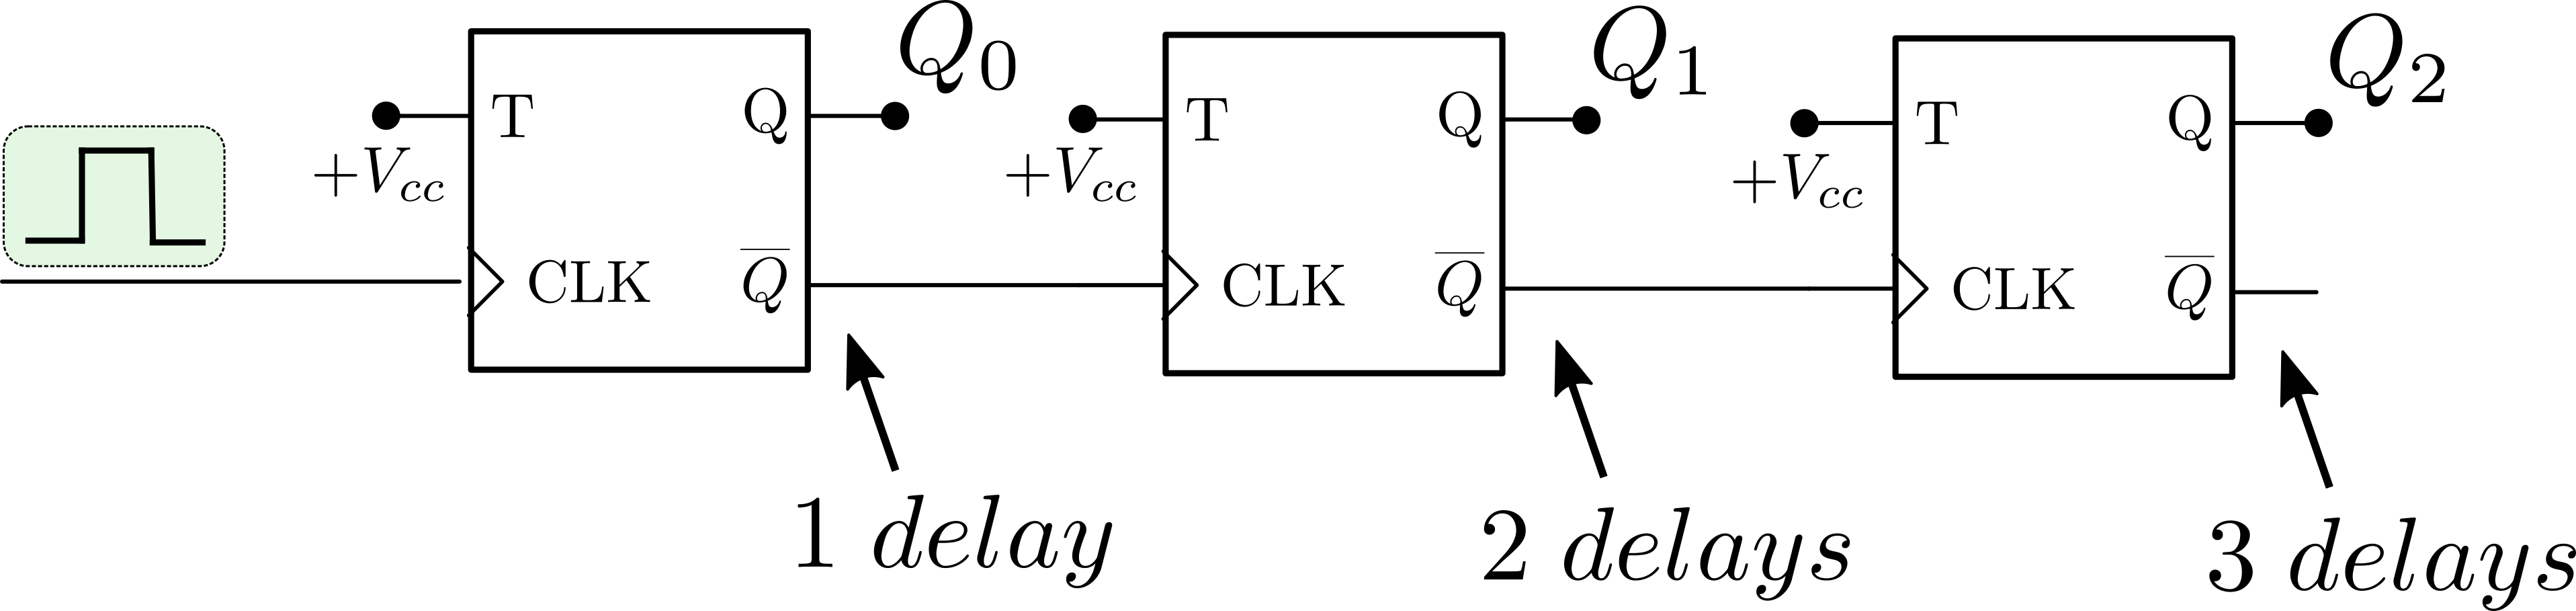
\includegraphics[width=1\textwidth]{data/async.png}
    \par\end{centering}
    \caption{Async. counter - delays}
\end{figure}


This counter work with a casquade triggering flip flops clocks done by the not Q output.

The idea is that, everytime the left flip flop is clocked two times, not Q goes up one time, thus, right flip flop is clocked one time (the half)
Propagating this logic to the general case, n-th flip flop has a period $2^n$ thus we made a binary counter. 

The theorical problem of this system is the delay propagation. As there is a delay between clock rising edge and Q update, the total delay will be multiplied by the number of flip flops.

\subsection*{Sync. counter}
\begin{figure}[H]
    \begin{centering}
    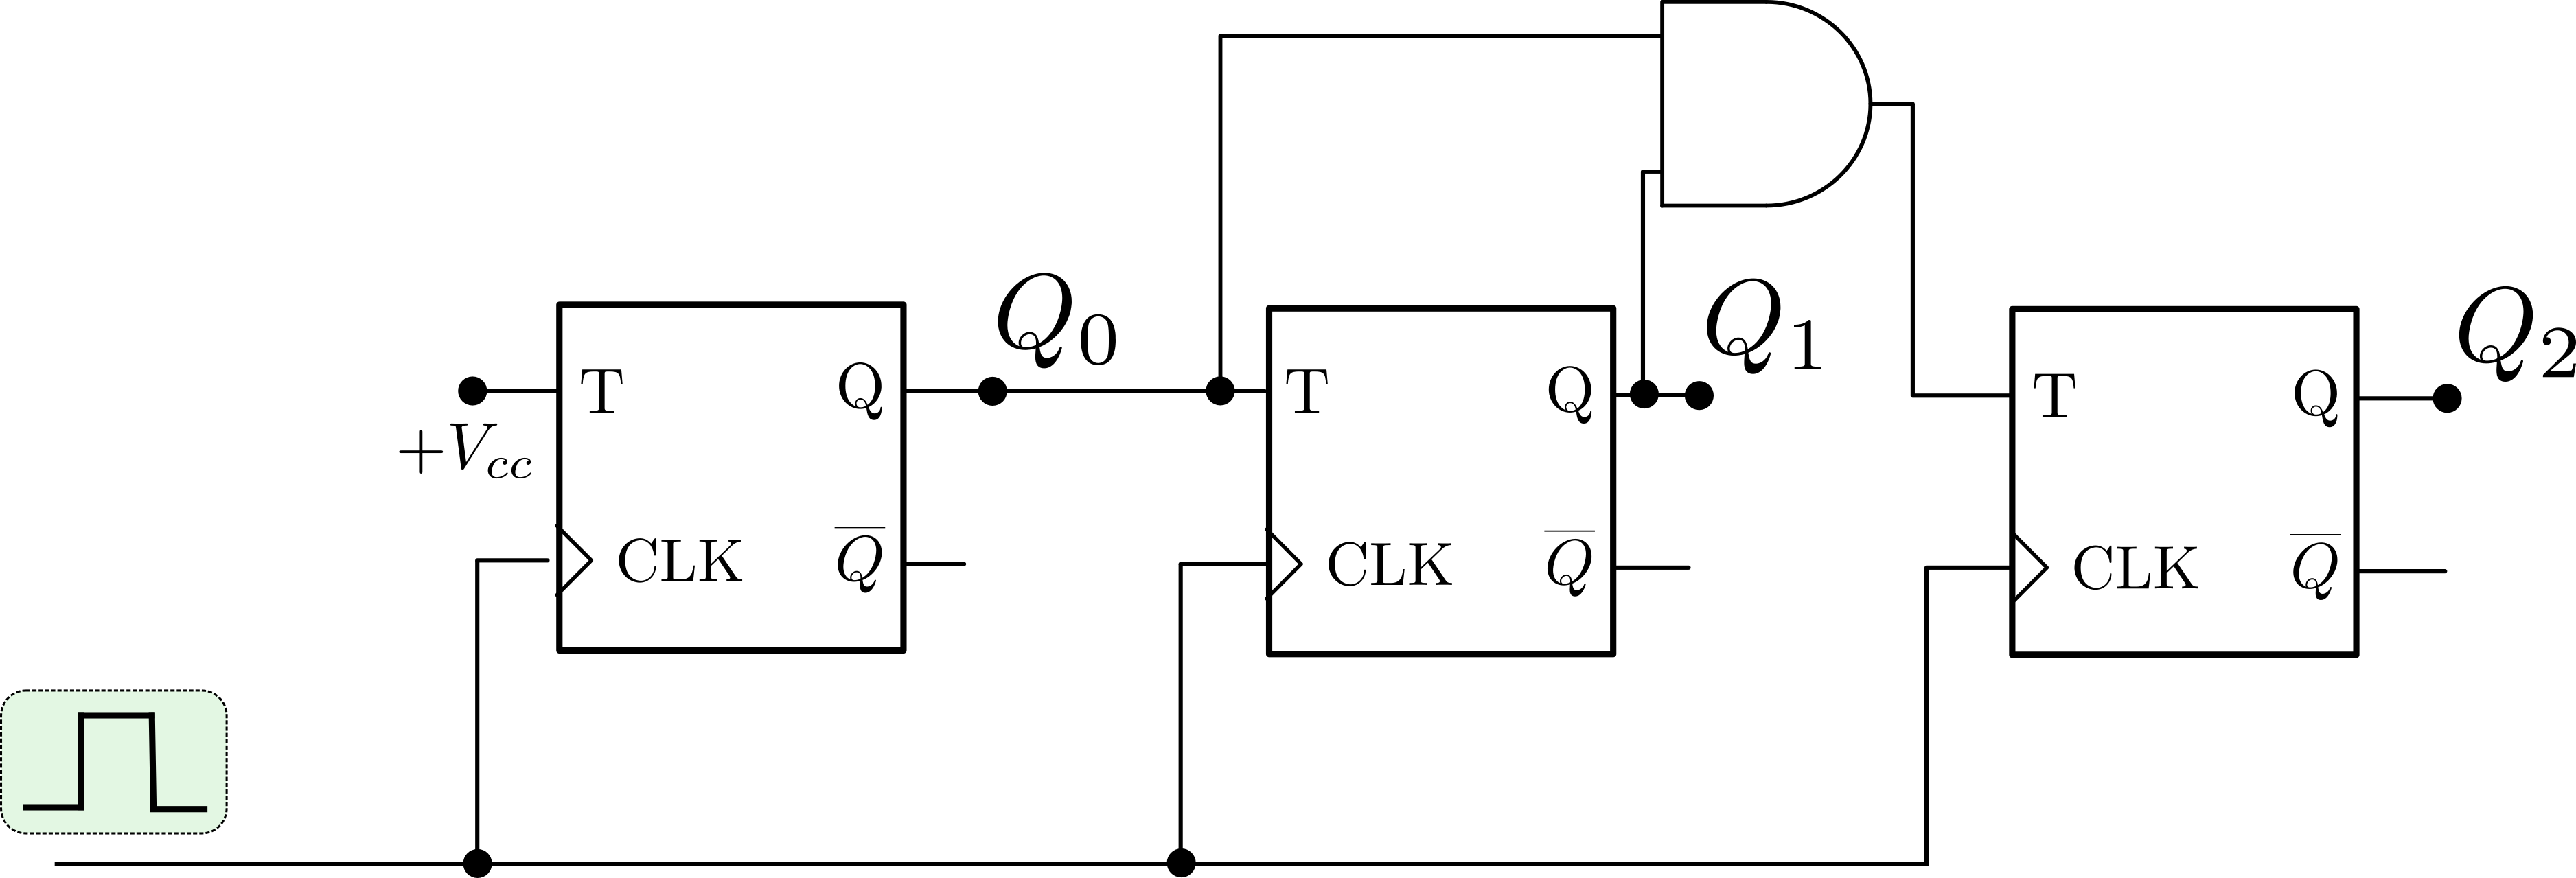
\includegraphics[width=1\textwidth]{data/sync.png}
    \par\end{centering}
    \caption{Sync. counter - delays}
\end{figure}

This counter is made to fix the problem of the previous counter. In this logic, all flip flops clocks are connected to the same trigger, thus, all of them are updated in the same instant, not, one after the other
